\chapter{Sequence Alignment}
\label{chap:seqal}

Il problema del Sequence Alignment consiste nel riuscire a comparare
delle stringhe, come per esempio quando si effettua un
\textbf{\emph{typo}} in un motore di ricerca e quello ci fornisce
l'alternativa corretta in quanto il testo da noi scritto è
``abbastanza'' simile a un'altra ricerca (che sia stata fatta con più
probabilità).\\ Vogliamo quindi un modello in cui la \textbf{similarità}
sia determinata approssimativamente dal numero di \textbf{gap} e
\textbf{mismatch} in cui incorriamo quando allineiamo le due parole.\\
Tuttavia ci sono varie possibilità con cui due parole di lunghezza
diversa possono essere confrontate, quindi è necessario fornire una
definizione di \textbf{similarità}.

\section{Descrizione del Problema}

Come prima definizione di \textbf{\emph{similarità}} possiamo dire che:

\begin{myblockquote}
  \begin{minipage}{\textwidth}
    \begin{definition}[\textbf{Similarità}]
      Minore è il numero di caratteri che non
      corrispondono, maggiore è la similarità tra le parole.
    \end{definition}
  \end{minipage}
\end{myblockquote}

Questa problematica è anche un tema centrale della biologia molecolare,
e proprio grazie ad un biologo abbiamo una definizione rigorosa e
soddisfacente di similarità.\\

Prima di dare una definizione similarità dobbiamo però darne una di
\textbf{allineamento}:
\newpage

\begin{myblockquote}
  \begin{minipage}{\textwidth}
    \begin{definition}[\textbf{Alignment}]
      Supponiamo di avere due stringhe
      $X$ e $Y$, che consistono rispettivamente della sequenza di simboli
      $x_1 x_2 \ldots x_m$ e $y_1 y_2 \ldots y_n$.
      Consideriamo gli insiemi $\{1,2,\ldots ,m\}$ e $\{1,2,\ldots ,n\}$
      che rappresentano le varie posizioni nelle stringhe $X$ e $Y$, e
      consideriamo un \textbf{Matching} di questi due insiemi (un matching è
      stato definito nel \autoref{chap:rna}
      $\rightarrow$ si tratta di un insieme di coppie ordinate con la
      proprietà che ogni oggetto si trova al più in una sola coppia).
      Diciamo ora che \textbf{un matching $M$ di questi due
        insiemi è un \emph{allineamento} se gli elementi di varie coppie non si
        incrociano}:
      \begin{itemize}
        \item se $(i,j),(i^{\prime},j^{\prime}) \in M$
        \item e $i < i^{\prime}$,
        \item allora $j < j^{\prime}$.
      \end{itemize}
    \end{definition}
  \end{minipage}
\end{myblockquote}

Intuitivamente, un \textbf{\emph{alignment}} fornisce un modo per
allineare le due stringhe, dicendoci quali coppie di posizioni saranno
allineate l'una con l'altra. Ad esempio:

\begin{verbatim}
stop-
-tops
\end{verbatim}

corrisponde all'alignment \texttt{\{(2,\ 1),\ (3,\ 2),\ (4,\ 3)\}}.\\

Ora la nostra definizione di similarità si baserà sul \textbf{trovare il
  miglior allineamento}, seguendo questi criteri:\\

Supponiamo che $M$ sia un dato allineamento tra $X$ e $Y$.

\begin{itemize}
  \item
        C'è un parametro $\delta>0$ che definisce la \textbf{gap penalty},
        che viene sostenuta ogni volta che un carattere di $X$ o $Y$ non è
        in un matching (ovvero non ha una corrispondenza). Nell'alignment il
        ``\textbf{\emph{gap}}'' viene posto con il simbolo `\texttt{-}',
        necessario al fine di allineare le due stringhe (avere uguale
        \emph{lunghezza}).
        \begin{center}
          \texttt{o-currance}\\
          \texttt{occurrance}
        \end{center}
  \item
        Per ogni coppia di lettere $p,q$ del nostro alfabeto, se c'è un
        accoppiamento errato si paga il corrispondente \textbf{mismatch cost}
        $a_{(p,q)}$.
        \begin{center}
          \texttt{occurrAnce}\\
          \texttt{occurrEnce}
        \end{center}
\end{itemize}


Il costo di $M$ è la somma del suo gap e mismatch cost, e
l'\textbf{obiettivo sarà quello di minimizzarlo}.

\paragraph*{Nota:} Le quantità $\delta$ e $a_{(p,q)}$ sono parametri
esterni che devono essere inseriti nel software per l'allineamento della
sequenza; infatti, molto lavoro va nella scelta delle impostazioni per
questi parametri. Dal nostro punto di vista, nel progettare un algoritmo
per il sequence alignment, li prenderemo come input.

\subsection{Goal}
\begin{myblockquote}
  \textbf{Date due stringhe, trovare l'allineamento di costo minimo.}
\end{myblockquote}

\paragraph*{Esempio:} data le parole \texttt{ocurrance} e
\texttt{occurrence} possiamo individuare vari alignment:

\begin{verbatim}
o-currAnce
occurrEnce
\end{verbatim}

oppure

\begin{verbatim}
o-curr-ance
occurre-nce
\end{verbatim}

Possiamo notare che nel primo abbiamo \textbf{1 gap} e \textbf{1
  mismatch} mentre nel secondo abbiamo \textbf{3 gap} ma \textbf{nessun
  mismatch}.\\
Vogliamo quindi determinare quale dei due sia il migliore.

\section{Implementazione dell'algoritmo}

Ora affronteremo il problema di calcolarci questo costo minimo, e
l'allineamento ottimale che lo fornisce, date le coppie $X$ e $Y$.\\
Come al solito proveremo con un approccio di programmazione dinamica, e
per realizzare l'algoritmo definiamo, come per altri algoritmi già
visti, una \textbf{scelta binaria}.\\ Dato l'allineamento ottimale $M$,
allora:
\begin{itemize}
  \item $(m,n) \in M$ (quindi gli ultimi due simboli delle due
        stringhe \textbf{sono in un matching})
  \item $(m,n) \notin M$ (gli ultimi
        simboli delle due stringhe \textbf{\emph{non} sono in un matching})
\end{itemize}

Tuttavia questa semplice distinzione \textbf{non è sufficiente}, quindi
supponiamo di aggiungere anche il seguente concetto elementare:
\begin{myblockquote}
  Sia $M$ un qualsiasi allineamento di $X$ e $Y$. Se $(m,n) \notin M$, allora,
  o l'$m$-esima posizione di $X$ o l' $n$-esima posizione di $Y$ \textbf{non è
    in un matching di $M$}.
\end{myblockquote}

Dire questo, equivale a riscrivere le due condizioni sopra come tre,
dunque \textbf{in un allineamento ottimo $M$ almeno una deve essere
  vera}:
\begin{enumerate}
  \item $(m,n) \in M$;
  \item l' $m-esima$ posizione di $X$ non è nel matching;
  \item l' $n-esima$ posizione di $Y$ non è nel matching
\end{enumerate}

Ora definiamo la funzione di costo minimo $OPT(i,j)$ come costo
dell'alignment tra $x_1 x_2 \ldots x_i$ e $y_1 y_2 \ldots y_j$.

\begin{itemize}
  \item
        \texttt{Nel\ caso\ 1}, abbiamo un costo di $a_{x_m y_n}$ e poi si
        allinea $x_1 x_2 \ldots x_{m-1}$ nel miglior modo possibile con
        $y_1 y_2 \ldots y_{n-1}$. Si ha quindi che
        $OPT(m,n) = a_{x_m y_n} + OPT(m-1,n-1)$.
  \item
        \texttt{Nel\ caso\ 2}, si paga un gap cost $\delta$ dato che la
        $m^{th}$ posizione di $X$ non è in matching, e poi si allinea
        $x_1 x_2 \ldots x_{m-1}$ nel miglior modo possibile con
        $y_1 y_2 \ldots y_{n}$. Si ha quindi che
        $OPT(m,n) = \delta + OPT(m-1,n)$.
  \item
        Similmente per \texttt{il\ caso\ 3}, abbiamo
        $OPT(m,n) = \delta + OPT(m,n-1)$.
\end{itemize}

Utilizzando dunque gli stessi argomenti per i sottoproblemi, per
l'allineamento di costo minimo tra $X$ e $Y$, otteniamo la
definizione generale di $OPT(i,j)$:

\begin{myblockquote}
  L'allineamento di costo minimo soddisfa la seguente ricorsione per
  $i \geq 1$ e $j \geq 1$:\\
  $OPT(i,j) = \min(a_{(x_i y_j)} + OPT(i-1, j-1), \delta + OPT(i-1, j), \delta + OPT(i, j-1))$
\end{myblockquote}

Dunque così abbiamo ottenuto la nostra funzione di ricorsione e possiamo
procedere alla scrittura dello pseudo codice sfruttando la
programmazione dinamica.

\subsection{Approccio Bottom-Up}

\begin{minipage}{\textwidth}
  \begin{lstlisting}[language=Python, mathescape=true]
function alignment(X,Y) {
	for i = 0 to m
		M[i, 0] $\leftarrow$ i $\delta$
	for j = 0 to n
		M[0, j] $\leftarrow$ j $\delta$
	for i = 1 to m
		for j = 1 to n
			M[i, j] $\leftarrow$ min (
				$\alpha$(xi yj) + M[i - 1, j - 1],
				$\delta$ + M [i - 1, j],
				$\delta$ + M [i, j - 1])

	return M[m, n]
}
\end{lstlisting}
\end{minipage}

\subsection{Costo}

\begin{itemize}
  \item
        Il running time è di $O(mn)$, poiché l'array $A$ ha $O(mn)$ voci
        e nel peggiore dei casi trascorriamo un tempo costante su ciascuna.
  \item
        Costo spaziale è di $O(mn)$
\end{itemize}

C'è un modo pittorico accattivante in cui le persone pensano a questo
algoritmo di sequence alignment. Supponiamo di costruire un grafo a
griglia $m$ \times $n$ bidimensionale $G_{XY}$ , con le righe
etichettate da simboli nella stringa $X$, le colonne etichettate da
simboli in $Y$ e gli archi orientati come nella \emph{Figura} di
seguito.

\begin{figure}[H]
  \begin{subfigure}{\textwidth}
    \centering
    \begin{subfigure}{.5\textwidth}
      \centering
      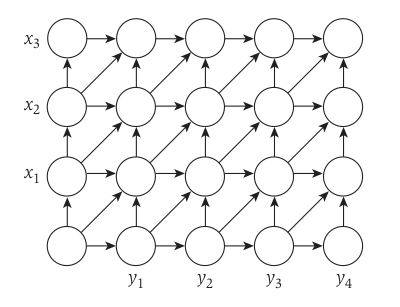
\includegraphics[width=\linewidth, keepaspectratio]{capitoli/programmazione_dinamica/imgs/sa.png}
    \end{subfigure}%
    \begin{subfigure}{.5\textwidth}
      \centering
      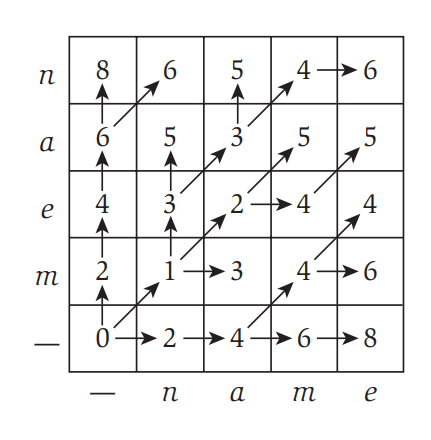
\includegraphics[width=.8\linewidth, keepaspectratio]{capitoli/programmazione_dinamica/imgs/seqalignmatrix.png}
    \end{subfigure}%
  \end{subfigure}
  \caption{Esempio di matching tra le parole \texttt{name} e \texttt{mean}.
    (Le due immagini si riferiscono ad esempi diversi.)}
\end{figure}

Nell'esempio precedente, il matching tra \texttt{name} e \texttt{mean}, con i
parametri scelti per questo esempio sarà:

\begin{verbatim}
mean-
n-ame
\end{verbatim}

Numeriamo le righe da 0 a $m$ e le colonne da 0 a $n$; indichiamo il
nodo nell'$i$-esima riga e nella $j$-esima colonna con l'etichetta
\texttt{(i,\ j)}. Mettiamo i costi sugli archi di $G_{XY}$ : il costo
di ogni arco orizzontale e verticale è $\delta$, e il costo dell'arco
diagonale da \texttt{(i\ -\ 1,\ j\ -\ 1)} a \texttt{(i,\ j)} è
$a_{x_i y_i}$.\\ Lo scopo di questa immagine emerge ora: la ricorrenza
definita precedentemente per $OPT(i, j)$ \textbf{è precisamente la
  ricorrenza che si ottiene per il percorso di costo minimo in $G_{XY}$
  da \texttt{(0,\ 0)} a \texttt{(i,\ j)}}. Così possiamo mostrare che:
\begin{myblockquote}
  Sia $f(i, j)$ il costo minimo di un cammino da
  \texttt{(0,\ 0)} a \texttt{(i,\ j)} in $G_{XY}$ . Allora per ogni
  $i$, $j$, abbiamo $f(i, j) = OPT(i, j)$.
\end{myblockquote}

Quindi il valore dell'allineamento ottimale è la lunghezza dello
shortest path in $G_{XY}$ da \texttt{(0,\ 0)} a \texttt{(m,\ n)}.\\
(Chiameremo qualsiasi percorso in $G_{XY}$ da \texttt{(0,\ 0)} a
\texttt{(m,\ n)} un \emph{percorso da angolo ad angolo}.) Inoltre, gli
archi diagonali utilizzati in un percorso più breve corrispondono
esattamente alle coppie utilizzate in un allineamento di costo minimo.
Queste connessioni al problema del cammino minimo nel grafo $G_{XY}$
non producono direttamente un miglioramento del tempo di esecuzione per
il problema dell'allineamento di sequenza; tuttavia, aiutano la propria
intuizione per il problema e sono stati utili nel suggerire algoritmi
per varianti più complesse sul sequence alignment.

\section{Riepilogo}

\begin{itemize}
  \item
        Trovare il numero di operazioni da fare per allineare due sequenze
  \item
        $OPT[i,j] = \min (\alpha_{ij} + OPT[i-1,j-1], \delta + OPT[i, j-1], \delta + OPT[i-1, j])$
  \item
        Ho bisogno di una matrice $i \times j$ \textbf{TEMPO =} $O(nm)$
        (nella versione base dell'algoritmo)
  \item
        Per ogni sottoproblema faccio solo un controllo. Posso anche
        utilizzare una matrice con sole due righe o sole due colonne
        \textbf{SPAZIO =} $O(nm)$ (nella versione base dell'algoritmo)
  \item
        \textbf{Per costruire la soluzione} ho bisogno di una matrice dove
        salvo le operazioni fatte, posso risalire in diagonale.

        \begin{itemize}
          \item
                \textbf{SPAZIO =} $O(nm)$
          \item
                \textbf{TEMPO =} $O(n+m)$
        \end{itemize}
\end{itemize}

\section{Hirschberg's algorithm}

\subsection{Sequence Alignment in Spazio Lineare utilizzando la Dividi et Impera}

Come abbiamo appena visto l'algoritmo ha sia costo spaziale che
temporale uguale a $O(mn)$ e se come input consideriamo le parole
della lingua inglese non risulta essere un grande problema, ma se
consideriamo genomi con 10 miliardi di caratteri potrebbe verificarsi la
situazione di dover lavorare con array anche superiori ai 10 GB, il che
renderebbe questo approccio molto costoso o quasi infattibile da
applicare. Tuttavia, questo problema può essere risolto utilizzando un
approccio \textbf{divide et impera} che va a rendere lineare il costo
dello spazio, ovvero $\rightarrow$ $O(n + m)$\\

Per facilità di presentazione, descriveremo vari passaggi in termini di
cammini nel grafico $G_{XY}$, con l'equivalenza naturale al problema
dell'allineamento della sequenza. Pertanto, quando cerchiamo le coppie
in un allineamento ottimale, possiamo equivalentemente chiedere gli
archi in un percorso \emph{angolo-angolo} più breve in $G_{XY}$.
L'algoritmo stesso sarà una bella applicazione delle idee \emph{divide
  et impera}. Il punto cruciale della tecnica è l'osservazione che,
\textbf{se dividiamo il problema in più chiamate ricorsive, allora lo
  spazio necessario per il calcolo può essere riutilizzato da una chiamata
  all'altra}. Il modo in cui questa idea viene utilizzata, tuttavia, è
abbastanza sottile.

\subsection{Implementazione dell'algoritmo}

Come prima cosa definiamo un algoritmo
\texttt{Space\ Efficient\ Alignment}, che ci permette di trovare la
soluzione ottima utilizzando il minor spazio possibile.\\ Per farlo,
notiamo che la funzione $OPT$ dipende solamente da una colonna
precedente di quella che si sta analizzando, dunque basterà caricarsi in
memoria una matrice $m \times 2$, riducendo così il costo spaziale ad
$m$. Tuttavia utilizzando questo metodo \textbf{non è possibile
  ricavare l'alignment effettivo} perché \textbf{non si hanno informazioni
  sufficienti}.\\

Lo pseudo-codice dell'algoritmo appena definito è il seguente:

\begin{lstlisting}[language=Python, mathescape=true]
function Space-Efficient-Alignment(X,Y) {
    var B = Matrix(m, 2)
    Initialize B[i, 0]= $i\delta$ for each i // (just as in column 0 of M)

    for (j in 1...n) {
        B[0, 1]= $j\delta$ (since this corresponds to entry M[0, j])

        for (i in 1...m) {
            B[i, 1]= min($\alpha$xiyj + B[i - 1, 0],$\delta$ + B[i - 1, 1], $\delta$ + B[i, 0])

        }

        Move column 1 of B to column 0 to make room for next iteration:
        Update B[i, 0]= B[i, 1] for each i
    }
}
\end{lstlisting}

Esiste, tuttavia, una soluzione a questo problema e saremo in grado di
recuperare l'allineamento stesso utilizzando lo spazio $O(m + n)$ ma,
richiede un'idea nuova. L'intuizione si basa sull'utilizzo della tecnica
\emph{divide et impera} che abbiamo visto in precedenza. Iniziamo con un
semplice modo alternativo per implementare la soluzione di
programmazione dinamica di base.

\paragraph{A Backward Formulation of the Dynamic Program:}\

Ricordiamo che
usiamo $f(i, j)$ per denotare la lunghezza del cammino minimo da
\texttt{(0,\ 0)} a \texttt{(i,\ j)} nel grafo $G_{XY}$. (Come abbiamo
mostrato nell'algoritmo di allineamento della sequenza iniziale,
$f(i, j)$ ha lo stesso valore di $OPT(i, j)$).\\ Ora definiamo
$g(i, j)$ come la lunghezza del cammino minimo da \texttt{(i\ ,\ j)} a
\texttt{(m,\ n)} in $G_{XY}$.\\ La funzione $g$ fornisce un approccio
di programmazione dinamica altrettanto naturale al problema del sequence
alignment, tranne per il fatto che \textbf{lo costruiamo al contrario}:
iniziamo con $g(m, n) = 0$ e la risposta che vogliamo è $g(0, 0)$.
Per stretta analogia con la ricorrenza precedente, abbiamo la seguente
ricorrenza per $g$:
\begin{myblockquote} Per $i < m$ e $j < n$ abbiamo:
  \begin{center}
    $g(i, j) = \min(a_{x_{i+1} y_{i+1}} + g(i + 1, j + 1), \delta + g(i, j + 1), \delta + g (i + 1, j))$
  \end{center}
\end{myblockquote}

Questa è solo la ricorrenza che si ottiene prendendo il grafo $G_{XY}$
, ``ruotandolo'' in modo che il nodo \texttt{(m,\ n)} si trovi
nell'angolo in basso a sinistra, e utilizzando l'approccio precedente.
Usando questa immagine, possiamo anche elaborare l'intero algoritmo di
programmazione dinamica per costruire i valori di $g$, a ritroso
partendo da \texttt{(m,\ n)}. Allo stesso modo, esiste una versione
efficiente in termini di spazio di questo algoritmo di programmazione
dinamica all'indietro, analogo a \texttt{Space-Efficient-Alignment}, che
calcola il valore dell'allineamento ottimale utilizzando solo lo spazio
$O(m+n)$. Faremo riferimento a questa versione all'indietro
come \texttt{Backward-Space-Efficient-Alignment}.\\

\paragraph*{Combinazione delle formulazioni Forward e Backward:}\
Quindi ora
abbiamo algoritmi simmetrici che costruiscono i valori delle funzioni
$f$ e $g$. L'idea sarà quella di utilizzare questi due algoritmi
insieme per trovare l'allineamento ottimale. Innanzitutto, ecco due
fatti fondamentali che riassumono alcune relazioni tra le funzioni $f$
e $g$.
\begin{myblockquote}
  La lunghezza del cammino \emph{angolo-angolo}
  più corto in $G_{XY}$ che passa per \texttt{(i, j)} è
  $f(i, j) + g(i, j)$.
\end{myblockquote}
\begin{myblockquote}
  Sia k un qualsiasi numero in ${0, . . . , n}$, e sia $q$ un indice
  che minimizza la quantità $f(q, k) + g(q, k)$. Poi c'è un percorso
  \emph{angolo-angolo} di lunghezza minima che passa attraverso il nodo \texttt{(q, k)}.
\end{myblockquote}

Possiamo sfruttare questo fatto per provare ad utilizzare lo
\texttt{Space\ Efficient\ Sequence\ Alignment\ Algorithm} combinato ad
un approccio \emph{\textbf{divide et impera}} e \textbf{un array di
  supporto $P$ per riuscire a calcolare il Sequence Alignment in spazio
  lineare}, aumentando solo di una costatane la complessità temporale.

\begin{lemma}
  $f(i,j) =$ shortest path from $(0,0)$ to
  $(i,j) = OPT(i,j)$
\end{lemma}
\begin{proof}
  Dimostriamo il lemma per induzione:

  \begin{itemize}
    \item caso base:
          $f(0,0) = OPT(0,0) = 0$
    \item ipotesi induttiva: assumo vero per ogni
          $(i', j')$ con $i'+j' < i+j$
    \item l'ultimo arco nello shortest path
          verso $(i,j)$ è $(i-1, j-1)$, $(i, j-1)$ o $(i-1, j)$
    \item quindi
          $f(i,j) = min\{ \alpha_{x_i y_j} + f(i-1, j-1), \delta + f(i-1, j), \delta +f(i, j-1)\} =$
          $= min\{ \alpha_{x_i y_j} + OPT(i-1, j-1), \delta + OPT(i-1, j), \delta + OPT(i, j-1)\} =$
          $= OPT(i,j)$
  \end{itemize}
\end{proof}

Per calcolare lo shortest path da un $(i,j)$ a $(m,n)$ posso
cambiare la direzione degli archi e calcolare lo shortest path da
$(m,n)$ a tutti i vertici $(i,j)$.\\
Il costo per andare da $(0,0)$ a $(m,n)$ posso scomporlo da
$(0,0)$ a $(i,j)$ e da $(m,n)$ a $(i,j)$.\\
Nel cammino incontrerò per forza la colonna $n/2$ ma non so per quale
vertice (riga $q$), voglio quindi trovarlo.
Divido quindi il problema in 2:

$$
  f((0,0)(q,n/2)) + f((q,n/2)(m,n))
$$

Così facendo posso quindi renderlo ricorsivo e durante
ogni ricorsione mi ricordo solo $q$.

\subsection{Funzionamento Algoritmo}

Dividiamo $G_{XY}$ lungo la sua colonna centrale e calcoliamo il
valore di $f(i, n/2)$ e $g(i, n/2)$ per ogni valore di $i$, usando
i nostri due algoritmi efficienti in termini di spazio. Possiamo quindi
determinare il valore minimo di $f(i, n/2) + g(i, n/2)$, e concludere
tramite la precedente definizione che esiste un cammino
\emph{angolo-angolo} più breve che passa attraverso il nodo
\texttt{(i,\ n/2)}. Detto questo, possiamo cercare ricorsivamente il
cammino minimo nella porzione di $G_{XY}$ tra \texttt{(0,\ 0)} e
\texttt{(i,\ n/2)} e nella porzione tra \texttt{(i,\ n/2)} e
\texttt{(m,\ n)}. Il punto cruciale è che applichiamo queste chiamate
ricorsive in sequenza e riutilizziamo lo spazio di lavoro da una
chiamata all'altra. Pertanto, poiché lavoriamo solo su una chiamata
ricorsiva alla volta, l'utilizzo totale dello spazio è $O(m + n)$. La
domanda chiave che dobbiamo risolvere è se il tempo di esecuzione di
questo algoritmo rimane $O(mn)$.\\ Nell'eseguire l'algoritmo, manteniamo
un elenco $P$ accessibile a livello globale che manterrà i nodi sul
percorso \emph{angolo-angolo} più breve man mano che vengono scoperti.\\
Inizialmente $P$ è vuoto. $P$ deve avere solo $m + n$ voci, poiché
nessun percorso da angolo a angolo può utilizzare più di questo numero
di archi. Usiamo anche la seguente notazione:\\ $X[i : j]$, per
$1 \le i \le j \le m$, denota la sottostringa di $X$ costituita da
$x_i x_{i+1} ... x_j$;\\ e definiamo $Y[i : j]$ in modo analogo.
Assumeremo per semplicità che $n$ sia una potenza di 2; questo
presupposto rende il discorso molto più pulito, anche se può essere
facilmente evitato.\\

Per prima cosa calcolo shortest path su tutta la matrice (Dijkstra in
$O(nm)$). Cerco poi $q$ sulla colonna $n/2$ e lo salvo
ricorsivamente $n$ volte.\\ Chiamo poi ricorsivamente $f$ per trovare
le soluzioni da sinistra a $n/2$ e da destra a $n/2$.\\

Possiamo riassumere il tutto con il seguente pseudo-codice:

\begin{lstlisting}[language=Python, mathescape=true]
function Divide-and-Conquer-Alignment(X,Y) {
    var m = length(X)
    var n = length(Y)

    if (m <= 2 or n <= 2) {
        Compute optimal alignment using Alignment(X,Y)
    }
    
    Space-Efficient-Alignment(X, Y[1 : n/2])
    Backward-Space-Efficient-Alignment(X, Y[n/2 + 1 : n])

    Let q be the index minimizing f(q, n/2) + g(q, n/2)
    Add (q, n/2) to global list P

    Divide-and-Conquer-Alignment(X[1 : q],Y[1 : n/2])
    Divide-and-Conquer-Alignment(X[q + 1 : n],Y[n/2 + 1 : n])
    
    return P
}
\end{lstlisting}

\begin{figure}[H]
  \centering
  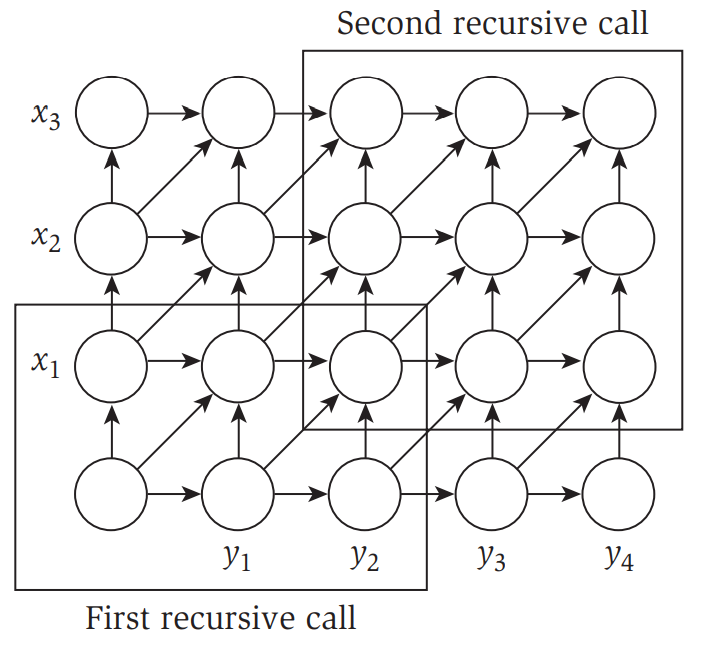
\includegraphics[width=10cm, keepaspectratio]{capitoli/programmazione_dinamica/imgs/seq_align_recurrence.png}
\end{figure}

\subsection{Costo}

$T(m,n) \le 2T(m, n/2) + O(nm) = O(mn \log n) \rightarrow$ Costo
troppo elevato.\\ I due sottoinsiemi però non sono $2T(m, n/2)$ ma
$(q, n/2) + (m-q, n/2)$

\begin{figure}[H]
  \centering
  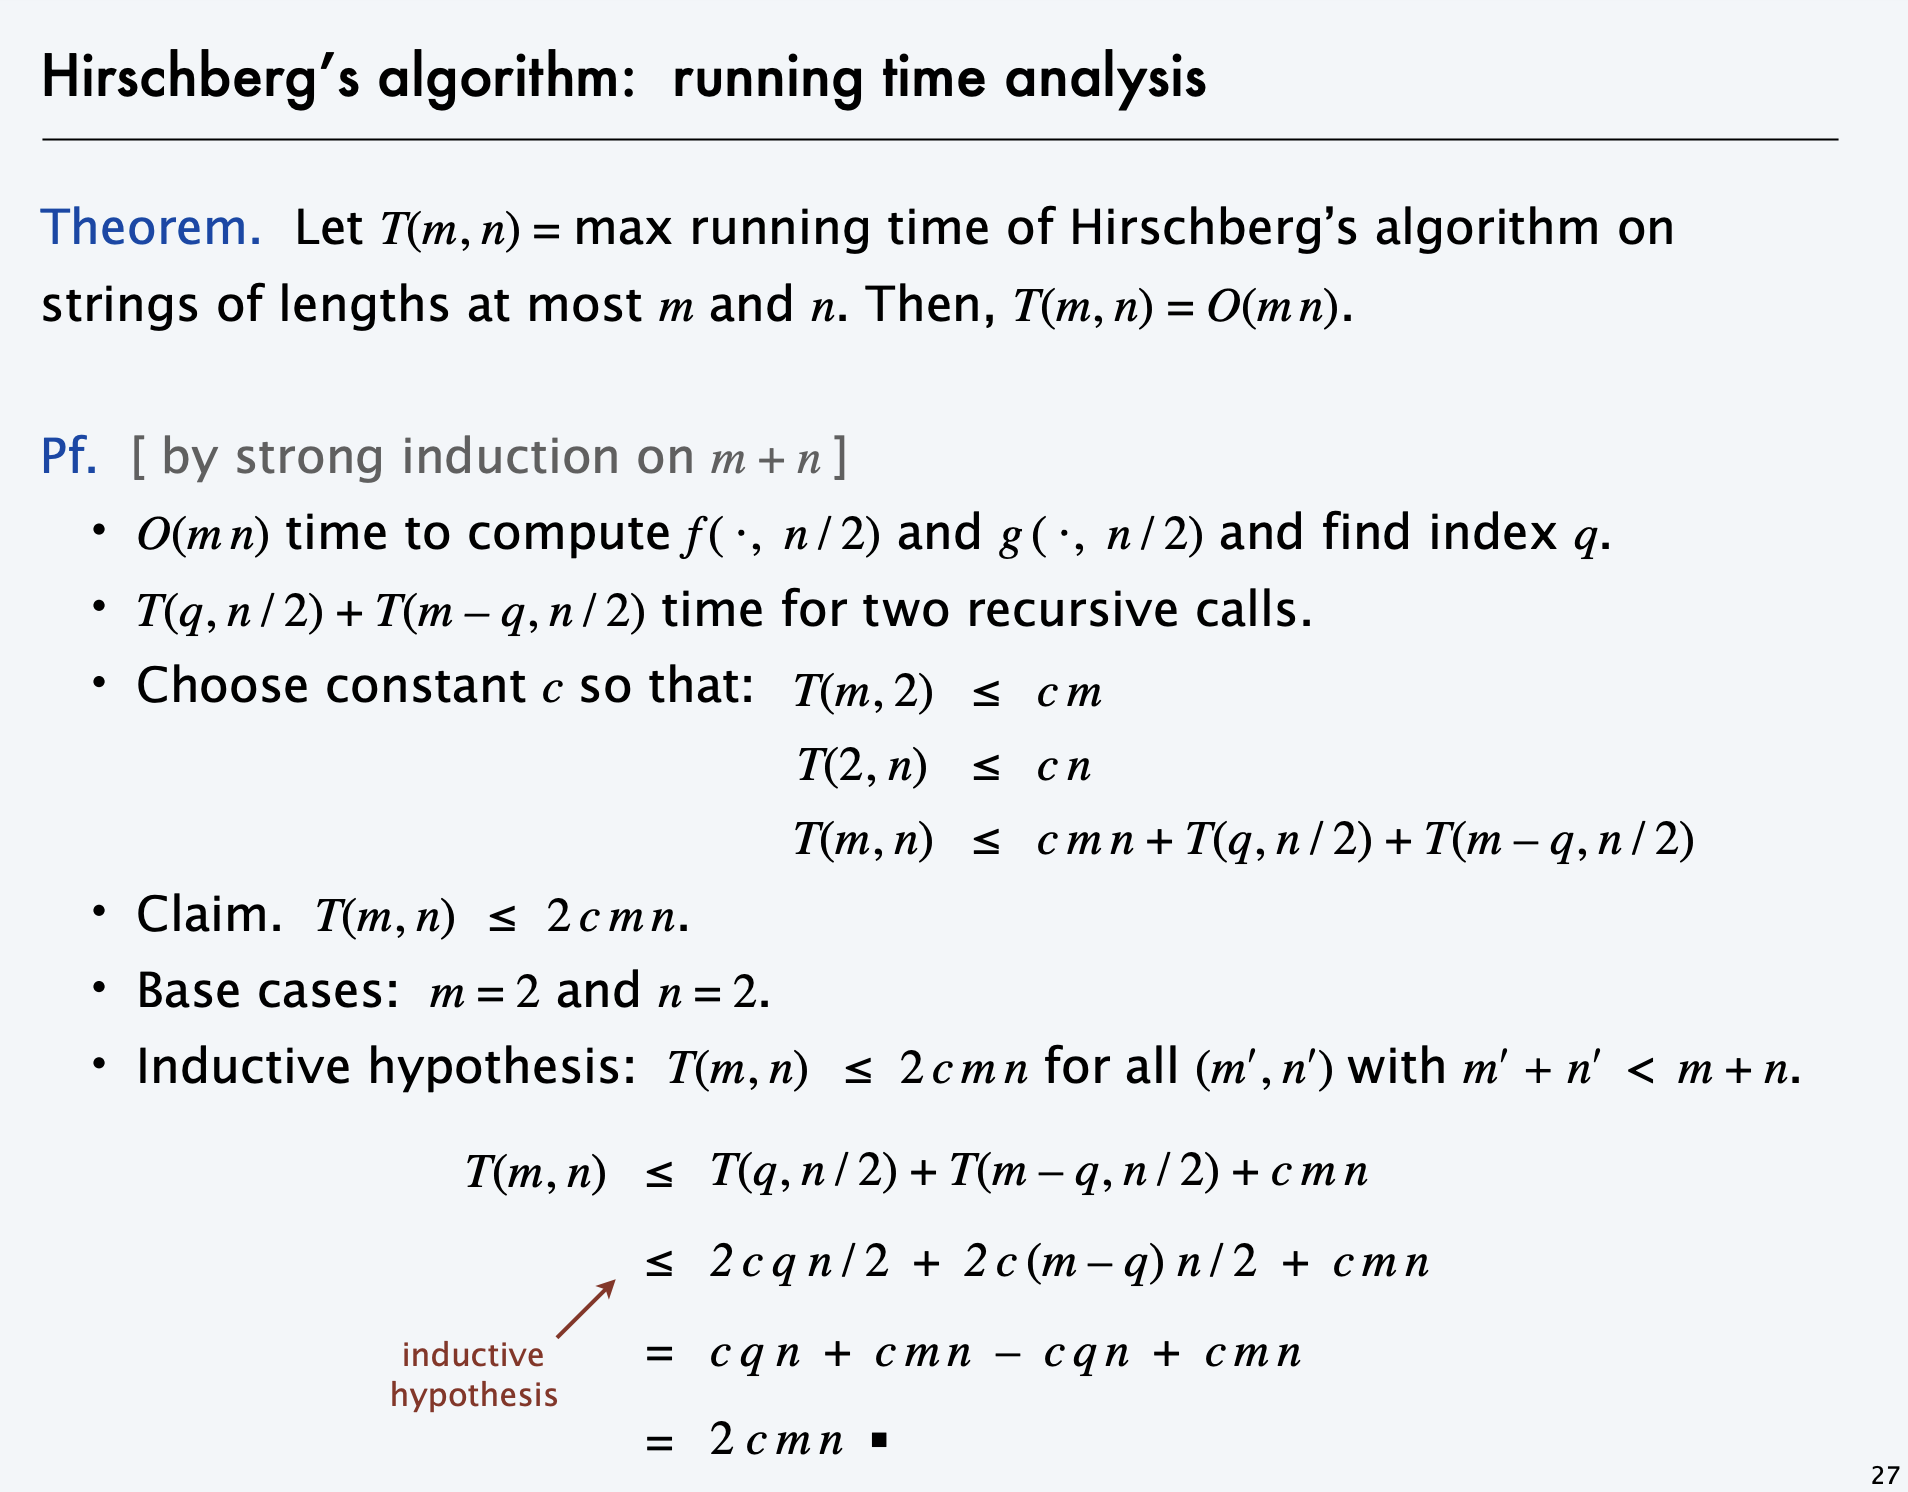
\includegraphics[width=12cm, keepaspectratio]{capitoli/programmazione_dinamica/imgs/hirschberg.png}
\end{figure}

Quindi, il tempo di esecuzione dell'alignment \emph{divide et impera} su
stringhe di lunghezza $m$ ed $n$ è $O(mn)$.

\section{Longest Common Subsequence}

È un caso particolare del problema del Sequence Alignment.

\subsection{Descrizione del Problema}

Per prima cosa è necessario dare la definizione di
\textbf{sottosequenza}. Una sottosequenza di una data sequenza è la
sequenza stessa alla quale sono stati tolti zero o più elementi.
Formalmente:\\

\begin{minipage}{\textwidth}
  \begin{myblockquote}
    Data una sequenza $X$ =
    $x_1, x_2, ..., x_m$, un'altra sequenza $Z$ = $z_1, z_2, ..., z_k$
    è una \textbf{sottosequenza} di $X$ se esiste una sequenza
    strettamente crescente $i_2, i_2, ..., i_k$ di indici di $X$ tale
    che per ogni $j = 1, 2, ..., k$, si ha $x_{i_j} = z_j$.
  \end{myblockquote}
\end{minipage}

Per esempio, $Z = <B, C, D, B>$ è una sottosequenza di
$X = < A, B, C, B, D, A, B>$ con la corrispondente sequenza di indici
$<2, 3, 5, 7>$.\\

Date due sequenze $X$ e $Y$, diciamo che una sequenza $Z$ è una
\textbf{sottosequenza comune} di $X$ e $Y$ se $Z$ è una
sottosequenza di entrambe le sequenze $X$ e $Y$. Per esempio, se
$X = <A,B,C,B,D,A,B>$ e $Y = <B,D,C,A,B,A>$, la sequenza $B,C,A$ è
una sottosequenza comune di $X$ e $Y$.

\paragraph*{Nota:} Il nostro obiettivo non è trovare una
sottosequenza comune, ma trovare la sottosequenza comune di lunghezza
massima.

\subsection{Goal}
\begin{myblockquote}
  Date due sequenze $X = <x_1, x_2, ..., x_m>$ e $Y = <y_1, y_2, ..., y_n>$
  trovare una sottosequenza di lunghezza massima che è comune a $X$ e $Y$.
\end{myblockquote}

\subsection{Caratterizzare la più lunga sottosequenza comune}

Una tecnica a forza bruta per risolvere questo problema consiste
nell'enumerare tutte le sottosequenze di $X$ e controllare le singole
sottosequenze per vedere se sono anche sottosequenze di $Y$. Un simile
approccio comporterebbe l'analisi di $2^m$ sottosequenze di $X$,
quindi questo approccio richiede un tempo esponenziale, il che lo rende
inutilizzabile per le sequenze lunghe.\\

Per costruire una rappresentazione che porta ad un approccio risolutivo
migliore, procediamo nel seguente modo: data una sequenza
$X = <x_1, x_2, ..., x_m>$, definiamo $X_i = <x_1, x_2, ..., x_i>$
l'$i$-esimo \textbf{prefisso} di $X$, per $i=0,1,...,m$. Per
esempio, se $X = <A,B,C,B,D,A,B>$, allora $X_4 = <A,B,C,B>$ e
$X_0$ è la sequenza vuota.

\begin{theorem}[\textbf{Sottostruttura ottima}]
  Siano $X = <x_1, x_2, ..., x_m>$ e $Y = <y_1, y_2, ..., y_n>$ le
  sequenze, sia $Z = z_1, z_2, ..., z_k$ una qualsiasi LCS di $X$ e
  $Y$.

  \begin{enumerate}
    \item Se $x_m = y_n$, allora $z_k = x_m = y_n$ e $Z_{k-1}$ è
          una LCS di $X_{m-1}$ e $Y_{n-1}$
    \item Se $x_m \ne y_n$, allora
          $z_k \ne x_m$ implica che $Z$ è una LCS di $X_{m-1}$ e $Y$.
    \item Se $x_m \ne y_n$, allora $z_k \ne y_n$ implica che $Z$ è una LCS
          di $X$ e $Y_{n-1}$.
  \end{enumerate}
\end{theorem}

Quindi, il problema della più lunga sottosequenza comune gode della
proprietà della sottostruttura ottima. Una soluzione ricorsiva gode
anche della proprietà dei sottoproblemi ripetuti.

\subsection{Soluzione Ricorsiva}

Il teorema precedente implica che ci sono uno o due sottoproblemi da
esaminare per trovare una LCS di $X = <x_1, x_2, ..., x_m>$ e $Y$ =
$<y_1, y_2, ..., y_n>$. Se $x_m = y_n$, dobbiamo trovare una LCS di
$X_{m-1}$ e $Y_{n-1}$. Accodando $x_m = y_n$ a questa LCS, si
ottiene una LCS di $X$ e $Y$. Se $x_m \neq y_n$, allora dobbiamo
risolvere due sottoproblemi: trovare una LCS di $X_{m-1}$ e $Y$ e
trovare una LCS di $X$ e $Y_{n-1}$. La più lunga di queste due LCS è
una LCS di $X$ e $Y$. Poiché questi casi esauriscono tutte le
possibilità, sappiamo che all'interno di una LCS di $X$ e $Y$ deve
essere utilizzata una delle soluzioni ottime dei sottoproblemi.\\

Come nel problema della moltiplicazione di una sequenza di matrici, la
nostra soluzione ricorsiva del problema della più lunga sottosequenza
comune richiede la definizione di una ricorrenza per il valore di una
soluzione ottima. Definiamo $c[i,j]$ come la lunghezza di una LCS
delle sequenze $X_i$ e $Y_j$. Se $i = 0$ o $j = 0$, una delle
sequenze ha lunghezza 0, quindi la LCS ha lunghezza 0. La sottostruttura
ottima del problema della LCS consente di scrivere la formula ricorsiva\\

$$
  c[i,j]= \begin{cases}
    0,                          & i = 0 \vee j = 0            \\
    c[i-1, j-1] + 1,            & i, j > 0 \wedge x_i = y_i   \\
    \max(c[i, j-1], c[i-1, j]), & i,j > 0 \wedge x_i \neq y_j
  \end{cases}
$$

\subsection{Calcolare la lunghezza di una LCS}

Utilizzando l'equazione precedente potremmo scrivere facilmente un
algoritmo ricorsivo con tempo esponenziale per calcolare la lunghezza di
una LCS di due sequenze. Tuttavia, poiché ci sono soltanto $O(mn)$
sottoproblemi distinti, posiamo utilizzare la programmazione dinamica
per calcolare le soluzioni con un metodo bottom-up. La procedura
\texttt{LCS-Length} riceve come input due sequenze
$X = <x_1, x_2, ..., x_m>$ e $Y$ = $<y_1, y_2, ..., y_n>$ e
memorizza i valori $c[i,j]$ in una tabella $c[0..m, 0..n]$, le cui
posizioni sono calcolate secondo l'ordine delle righe (cioè, vengono
inseriti i valori nella prima riga di $c$ da sinistra a destra, poi
vengono inseriti i valori nella seconda riga e così via).\\

La procedura utilizza anche la tabella $b[1..m, 1..n]$ per
semplificare la costruzione di una soluzione ottima. Intuitivamente,
$b[i, j]$ punta alla posizione della tabella che corrisponde alla
soluzione ottima del sottoproblema che è stata scelta per calcolare
$c[i,j]$. La procedura restituisce le tabelle $b$ e $c$; la
posizione $c[m,n]$ contiene la lunghezza di una LCS di $X$ e $Y$.\\

\begin{lstlisting}[language=Python, mathescape=true]
function LCS-Length(X, Y) {
  m = X.length
  n = Y.length

  Let b[1..m, 1..n] e c[0..m, 0..n] two new tables

  for i = 1 to m
    c[i,0] = 0

  for j = 0 to n
    c[0,j] = 0

  for i = 1 to m
    for j = 1 to n
      if xi == yi
        c[i,j] = c[i-1, j-1] + 1
        b[i,j] = $\nwarrow$
      elseif c[i-1,j] $\ge$ c[i,j-1]
        c[i,j] = c[i-1,j]
        b[i,j] = $\uparrow$
      else 
        c[i,j] = c[i,j-1] 
        b[i,j] = $\leftarrow$

  return c e b
}
\end{lstlisting}

\subsection{Costo}

Il tempo di esecuzione è $O(mn)$, perché il calcolo di ogni posizione
della tabella richiede un tempo $O(1)$

\subsection{Costruire una LCS}

La tabella $b$ restituita dalla procedura \texttt{LCS-length} può
essere utilizzata per costruire rapidamente una LCS delle sequenze
$X = <x_1, x_2, ..., x_m>$ e $Y$ = $<y_1, y_2, ..., y_n>$.
Iniziamo semplicemente da $b[m,n]$ e, ogni volta che incontriamo una
freccia $\nwarrow $ nella posizione $b[i,j]$, significa che $x_i = y_j$ è
un elemento della LCS trovata da \texttt{LCS-Length}. In questo modo gli
elementi della LCS si incontrano in ordine inverso. La seguente
procedura ricorsiva stampa una LCS di $X$ e $Y$ nell'ordine
corretto. La chiamata iniziale è
\texttt{Print-LCS(b,\ X,\ X.length,\ Y.length)}.\\

\begin{minipage}{\textwidth}
  \begin{lstlisting}[language=Python, mathescape=true]
function Print-LCS(b, X, i, j) {
    if i == 0 or j == 0
      return

    if b[i,j] == $\nwarrow $
      Print-LCS(b, X, i-1, j-1)
      print xi
    else if b[i,j] == $\uparrow$
      Print-LCS(b, X, i$-$1, j)
    else
      Print-LCS(b, X, i, j$-$1)
  }
\end{lstlisting}
\end{minipage}

La procedura impiega un tempo $O(m + n)$, perché a ogni chiamata
ricorsiva essa decrementa almeno uno dei due valori $i$ e $j$.
